\documentclass[letterpaper]{article}
\usepackage[margin=1in]{geometry}
\usepackage[utf8]{inputenc}
\usepackage{textcomp}
\usepackage{amssymb}
\usepackage{natbib}
\usepackage{graphicx}
\usepackage{gensymb}
\usepackage{amsthm, amsmath, mathtools}
\usepackage[dvipsnames]{xcolor}
\usepackage{enumerate}
\usepackage{mdframed}
\usepackage[most]{tcolorbox}
\usepackage{csquotes}
% https://tex.stackexchange.com/questions/13506/how-to-continue-the-framed-text-box-on-multiple-pages

\tcbuselibrary{theorems}

\newcommand{\R}{\mathbb{R}}
\newcommand{\Z}{\mathbb{Z}}
\newcommand{\N}{\mathbb{N}}
\newcommand{\Q}{\mathbb{Q}}
\newcommand{\C}{\mathbb{C}}
\newcommand{\code}[1]{\texttt{#1}}
\newcommand{\mdiamond}{$\diamondsuit$}
\newcommand{\PowerSet}{\mathcal{P}}
\newcommand{\Mod}[1]{\ (\mathrm{mod}\ #1)}
\DeclareMathOperator{\lcm}{lcm}

%\newtheorem*{theorem}{Theorem}
%\newtheorem*{definition}{Definition}
%\newtheorem*{corollary}{Corollary}
%\newtheorem*{lemma}{Lemma}
\newtheorem*{proposition}{Proposition}


\newtcbtheorem[number within=section]{theorem}{Theorem}
{colback=green!5,colframe=green!35!black,fonttitle=\bfseries}{th}

\newtcbtheorem[number within=section]{definition}{Definition}
{colback=blue!5,colframe=blue!35!black,fonttitle=\bfseries}{def}

\newtcbtheorem[number within=section]{corollary}{Corollary}
{colback=yellow!5,colframe=yellow!35!black,fonttitle=\bfseries}{cor}

\newtcbtheorem[number within=section]{lemma}{Lemma}
{colback=red!5,colframe=red!35!black,fonttitle=\bfseries}{lem}

\newtcbtheorem[number within=section]{example}{Example}
{colback=white!5,colframe=white!35!black,fonttitle=\bfseries}{def}

\newtcbtheorem[number within=section]{note}{Important Note}{
        enhanced,
        sharp corners,
        attach boxed title to top left={
            xshift=-1mm,
            yshift=-5mm,
            yshifttext=-1mm
        },
        top=1.5em,
        colback=white,
        colframe=black,
        fonttitle=\bfseries,
        boxed title style={
            sharp corners,
            size=small,
            colback=red!75!black,
            colframe=red!75!black,
        } 
    }{impnote}
\usepackage[utf8]{inputenc}
\usepackage[english]{babel}
\usepackage{fancyhdr}
\usepackage[hidelinks]{hyperref}

\pagestyle{fancy}
\fancyhf{}
\rhead{Math 170B}
\chead{Wednesday, April 26, 2023}
\lhead{Lecture 11}
\rfoot{\thepage}

\setlength{\parindent}{0pt}

\begin{document}

\section{Divided Differences (Section 6.2)}
We'll begin by briefly reviewing Newton's Form from the previous section. Recall the coefficients in the Newton form of interpolating polynomial, $P(x)$, where $f(x)$ is interpoled by $P(x)$, is $c_i$. Then, 
\[P(x_i) = \underbrace{f(x_i)}_{\text{Data}} \quad 0 \leq i \leq m.\]
Newton's Form looks like  
\[P(x) = c_0 + c_1 (x - x_0) + c_2 (x - x_0) (x - x_1) + \hdots + c_m (x - x_0) (x - x_1) \hdots (x - x_{m - 1}).\]
Then, 
\begin{equation}{\label{11:2}}
    \begin{aligned}
        P(x_0) &= f(x_0) = c_0 \\ 
        P(x_1) &= f(x_1) = c_0 + c_1 (x_1 - x_0) \\ 
        P(x_2) &= f(x_2) = c_0 + c_1 (x_2 - x_0) + c_2 (x_2 - x_0) (x_2 - x_1)
    \end{aligned}
\end{equation}
We can represent (\ref{11:2}) as a system of equations, modeled using matrices, like so: 
\[
    \begin{bmatrix}
        1 & 0 & 0 \\ 
        1 & (x_1 - x_0) & 0 \\  
        1 & (x_2 - x_0) & (x_2 - x_0)(x_2 - x_1)
    \end{bmatrix} \begin{bmatrix}
        c_0 \\ c_1 \\ c_2 
    \end{bmatrix} = \begin{bmatrix}
        f(x_0) \\ 
        f(x_1) \\ 
        f(x_2)
    \end{bmatrix}.
\]
This is a triangular system. We can represent the $c_i$'s in terms of the $f(x_i)$'s. Thus, the \textbf{divided difference} is defined by
\begin{equation}
    f[x_0, x_1, x_2, \hdots, x_m] \equiv c_m.
\end{equation}
We say that $f[x_0, x_1, x_2, \hdots, x_m]$ is the coefficient of $x^m$ in the polynomial of degree at most $n$ that interpolates $f$ at $x_0, x_1, \hdots, x_n$. With this in mind, some explicit formulas include 
\begin{itemize}
    \item if $m = 0$, then $c_0 = f[x_0] = f(x_0)$. 
    \item if $m = 1$, then $c_1 = f[x_0, x_1] = \frac{f(x_1) - f(x_0)}{x_1 - x_0}$.
\end{itemize}
Thus, the Newton interpolating form can be rewritten as 
\[P(x) = \sum_{k = 0}^{m} f[x_0, x_1, x_2, \hdots, x_k] \prod_{j = 0}^{k - 1} (x - x_j).\]

\subsection{Higher Order Differences}
\begin{theorem}{Divided Difference}{}
    Divided differences satisfy the equation,
    \[f[x_0, x_1, \hdots, x_m] = \frac{f[x_1, x_2, \hdots, x_m] - f[x_0, x_1, \hdots, x_{m - 1}]}{x_m - x_0}.\]
\end{theorem}

\begin{proof}
    Let $P_{k}(x)$ be a polynomial of degree at most $k$ interpolating $x_0, x_1, \hdots, x_k$. Further, let $Q_{k}(x)$ be a polynomial of degree at most $m - 1$ interpolating $x_1, x_2, \hdots, x_m$. Then, we have $P_{k}(x_i) - f(x_i)$ for $0 \leq i \leq k$ and $q(x_i) = f(x_i)$ for $1 \leq i \leq m$. So, 
    \[P_{m}(x) = q(x) + \frac{(x - x_m)}{x_m - x_0} (q(x) - P_{m - 1}(x)).\]
    We can verify that any data point we substitute in will satisfy the above equation. In any case, the left- and right-hand sides match at $x_0, x_1, \hdots, x_m$. Then, the coefficients on the left- and right- for $x^m$ are 
    \[f[x_0, x_1, \hdots, x_m] = \frac{f[x_1, x_2, \hdots, x_m] - f[x_0, x_1, \hdots, x_{m - 1}]}{x_m - x_0},\]
    as desired.
\end{proof}

So, with this formula, if we were to consider $m = 0$, then \[f[x_0] = f(x_0).\] Likewise, if we consider $m = 1$, we have \[f[x_0, x_1] = \frac{f[x_1] - f[x_0]}{x_1 - x_0}.\] Finally, for $m = 3$, we have \[f[x_0, x_1, x_2] = \frac{f[x_1, x_2] - f[x_0, x_1]}{x_2 - x_0}.\]

The recursive relation is given by 
\begin{equation}{\label{11:1}}
    f[x_i, x_{i + 1}, x_{i + 2}, \hdots, x_{i + j}] = \frac{f[x_{i + 1}, x_{i + 2}, \hdots, x_{i + j}] - f[x_i, x_{i + 1}, \hdots, x_{i + j - 1}]}{x_{i + j} - x_{i}}.
\end{equation}
We can describe this recursive relation in terms of a table. For a table of function values $(x_i, f(x_i))$, 
\begin{center}
    \begin{tabular}{c|c|c|c|c}
              & 0        & 1             & 2                  & 3 \\ 
            \hline 
        $x_0$ & $f(x_0)$ & $f[x_0, x_1]$ & $f[x_0, x_1, x_2]$ & $f[x_0, x_1, x_2, x_3]$ \\ 
        $x_1$ & $f(x_1)$ & $f[x_1, x_2]$ & $f[x_1, x_2, x_3]$ & \\ 
        $x_2$ & $f(x_2)$ & $f[x_2, x_3]$ &                    & \\ 
        $x_3$ & $f(x_3)$ &               &                    & \\ 
    \end{tabular}
\end{center}
Note that $f(x_i) = f[x_i]$. So, the top row of the table corresponds to the coefficients in Newton's form. Each columns represents the difference of orders. The recursive relationship is given by 
\begin{center}
    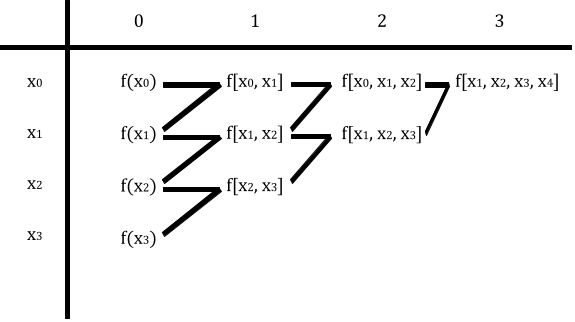
\includegraphics[scale=0.6]{../assets/divided_diff_functions.png}
\end{center}
For example, the calculation of $f[x_1, x_2, x_3]$ depends on the result of $f[x_1, x_2]$ and $f[x_2, x_3]$; to see why, from (\ref{11:1}), note that 
\[f[x_1, x_2, x_3] = \frac{f[x_2, x_3] - f[x_1, x_2]}{x_3 - x_1}.\]

\begin{mdframed}
    (Exercise.) Given the set of points, 
    \begin{center}
        \begin{tabular}{c||c c c c}
            $x$ & 3 & 1 & 5 & 6 \\ 
            \hline 
            $f(x)$ & 1 & -3 & 2 & 4
        \end{tabular}
    \end{center}
    Compute a divided difference table for these function values.

    \begin{mdframed}
        We have the table 
        \begin{center}
            \begin{tabular}{c||c c c c}
                $x_i$ & $f(x_i)$ &   &    &    \\ 
                \hline 
                $3$ & $1$ & $f[x_0, x_1]$ & $f[x_0, x_1, x_2]$ & $f[x_0, x_1, x_2, x_3]$ \\ 
                $1$ & $-3$ & $f[x_1, x_2]$ & $f[x_1, x_2, x_3]$ & \\ 
                $5$ & $2$ & $f[x_2, x_3]$ &                    & \\ 
                $6$ & $4$ &    
            \end{tabular}
        \end{center}
        Using the table above, we find that, 
        \begin{itemize}
            \item for the first column, i.e., $f[x_i, x_j]$, 
            \[f[x_0, x_1] = \frac{f[x_1] - f[x_0]}{x_1 - x_0} = \frac{f(x_1) - f(x_0)}{x_1 - x_0} = \frac{-3 - 1}{1 - 3} = \frac{-4}{-2} = 2.\]
            \[f[x_1, x_2] = \frac{f[x_2] - f[x_1]}{x_2 - x_1} = \frac{f(x_2) - f(x_1)}{x_2 - x_1} = \frac{2 - (-3)}{5 - 1} = \frac{5}{4}.\]
            \[f[x_2, x_3] = \frac{f[x_3] - f[x_2]}{x_3 - x_2} = \frac{f(x_3) - f(x_2)}{x_3 - x_2} = \frac{4 - 2}{6 - 5} = \frac{2}{1} = 2.\]

            \item for the second column, i.e, $f[x_i, x_j, x_k]$, 
            \[f[x_0, x_1, x_2] = \frac{f[x_1, x_2] - f[x_0, x_1]}{x_2 - x_0} = \frac{\frac{5}{4} - 2}{5 - 3} = -\frac{3}{8}.\]
            \[f[x_1, x_2, x_3] = \frac{f[x_2, x_3] - f[x_1, x_2]}{x_3 - x_1} = \frac{2 - \frac{5}{4}}{6 - 1} = \frac{3}{20}.\]

            \item for the third column, i.e., $f[x_i, x_j, x_k, x_\ell]$, 
            \[f[x_0, x_1, x_2, x_3] = \frac{f[x_1, x_2, x_3] - f[x_0, x_1, x_2]}{x_3 - x_0} = \frac{\frac{3}{20} - \left(-\frac{3}{8}\right)}{6 - 3} = \frac{7}{40}.\]
        \end{itemize}
        Therefore, the divided difference table looks like 
        \begin{center}
            \begin{tabular}{c||c c c c}
                $x_i$ & $f(x_i)$ &   &    &    \\ 
                \hline 
                $3$ & $1$ & $2$ & $-\frac{3}{8}$ & $\frac{7}{40}$ \\ 
                $1$ & $-3$ & $\frac{5}{4}$ & $\frac{3}{20}$ & \\ 
                $5$ & $2$ & $2$ &                    & \\ 
                $6$ & $4$ &    
            \end{tabular}
        \end{center}
        Recall that the top row of the table corresponds to the coefficients in Newton's form, so we find that the interpolating polynomial $P(x)$ is 
        \[\begin{aligned}
            P(x) &= c_0 + c_1 (x - x_0) + c_2 (x - x_0) (x - x_1) + c_3 (x - x_0) (x - x_1) (x - x_2) \\ 
                &= 1 + 2(x - 3) - \frac{3}{8}(x - 3)(x - 1) + \frac{7}{40}(x - 3)(x - 1)(x - 5)
        \end{aligned}.\]
    \end{mdframed}
\end{mdframed}


\end{document}